% Created 2019-10-15 Tue 21:45
% Intended LaTeX compiler: pdflatex
\documentclass[presentation]{beamer}
\usepackage[utf8]{inputenc}
\usepackage[T1]{fontenc}
\usepackage{graphicx}
\usepackage{grffile}
\usepackage{longtable}
\usepackage{wrapfig}
\usepackage{rotating}
\usepackage[normalem]{ulem}
\usepackage{amsmath}
\usepackage{textcomp}
\usepackage{amssymb}
\usepackage{capt-of}
\usepackage{hyperref}
\usepackage{lmodern}
\usetheme{default}
\date{October 17, 2019}
\title{Functionality Slices Working Group}
\hypersetup{
 pdfauthor={},
 pdftitle={Functionality Slices Working Group},
 pdfkeywords={},
 pdfsubject={},
 pdfcreator={Emacs 26.2 (Org mode 9.1.9)}, 
 pdflang={English}}
\begin{document}

\maketitle

\begin{frame}[label={sec:org09a55ee}]{Why?}
\begin{itemize}
\item \alert{Problem:} Given the size and structure of the PMIx standard document, it can be difficult to find the PMIx components necessary for a given use-case
\item \alert{Goal:} Provide a mechanism for focusing in on the aspects of the standard that are of interest to a particular user/use-case
\item \alert{Proposed solution:} compile a list of high-level use-cases and the PMIx capabilities required to support them
\end{itemize}
\end{frame}
\begin{frame}[label={sec:org6b17e15}]{Areas for Improvement}
\begin{itemize}
\item It’s not a quality problem, but quantity one
\begin{itemize}
\item \textasciitilde{}140 interfaces across \textasciitilde{}340 pages
\end{itemize}
\item The document is written primarily as an API reference
\item Some interfaces "wear lots of hats"
\begin{itemize}
\item PMIx\_Get, PMIx\_Job\_Control, etc
\end{itemize}
\end{itemize}
\end{frame}
\begin{frame}[label={sec:orga50bf20}]{Audience \& Questions We Want to Answer}
\begin{block}{Users of Client-Side Interfaces}
\begin{itemize}
\item I currently do X with some other interface/middleware, how do I do it with PMIx?
\item I currently use the baseline PMIx functionality to do X, are there other (better) ways to do it in PMIx?
\item I have some completely new use-case, can I mix-and-match existing PMIx functionality to meet my needs?
\end{itemize}
\end{block}
\begin{block}{Users of Server-Side Interfaces}
\begin{itemize}
\item What server-side interfaces are necessary to support a given client interface or high-level use-case?
\item What client-side interfaces are necessary to support a given high-level use-case?
\end{itemize}
\end{block}
\end{frame}
\begin{frame}[label={sec:org772bbd6}]{Goals}
\begin{block}{Short-term:}
\begin{itemize}
\item Use-Case Milestone 1 (Jan 2020):
\begin{itemize}
\item bootstrap (business card exchange)
\item debuggers / tools
\end{itemize}
\item Use-Case Milestone 2 (End of Q1 2020):
\begin{itemize}
\item instant-on
\item hybrid programming models
\item workflow management
\item application management
\end{itemize}
\end{itemize}
\end{block}
\end{frame}
\begin{frame}[label={sec:orgaeb1095}]{Goals}
\begin{block}{Long-term:}
\begin{itemize}
\item Identify and document emerging use-cases:
\begin{itemize}
\item tiered storage
\item power control
\item groups/flexible allocations
\item fault tolerance
\item cross-version compatibility
\end{itemize}
\item Determine how to handle “miscellaneous” interfaces
\item Document which resource managers support which use-cases
\item Add interfaces into the standard for querying "use-case support"
\end{itemize}
\end{block}
\end{frame}
\begin{frame}[label={sec:org1ed18dc}]{Work Completed So Far}
\begin{itemize}
\item Went through each RFC, documenting the interfaces and use-cases covered
\item Aggregated the RFC notes into rough slices
\item Analysis of what interfaces were not covered by RFCs
\item Drafts of Debugging \& Bootstrap Use-Cases
\begin{itemize}
\item Currently "issues" in the pmix/pmix-standard GitHub repo
\end{itemize}
\end{itemize}
\begin{center}
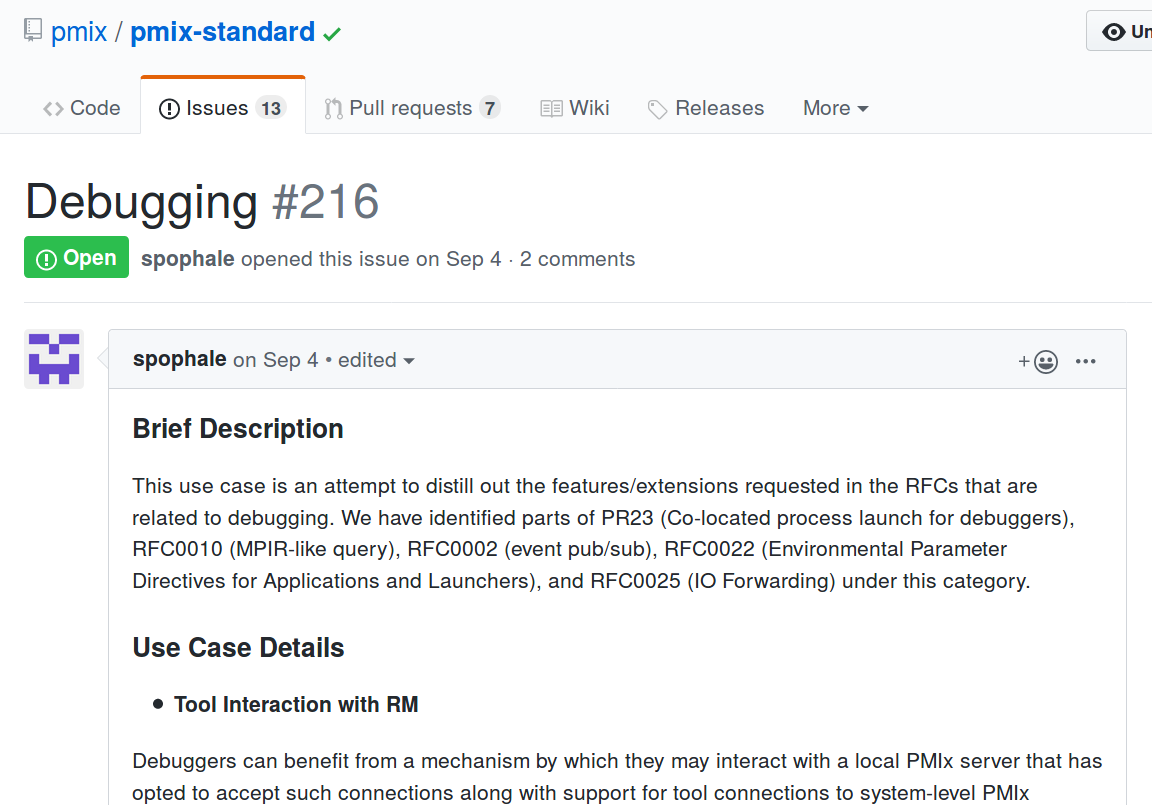
\includegraphics[width=.9\linewidth]{./figures/Debugging.png}
\end{center}
\end{frame}
\begin{frame}[label={sec:org4f50a64}]{Call for Participation}
\begin{block}{Works In Progress}
\begin{itemize}
\item General structure and template for Use-Cases
\item Hybrid Programming Models \& Instant-On Use-Cases
\item Coverage Analysis
\end{itemize}
\end{block}
\begin{block}{Help Wanted}
\begin{itemize}
\item Identifying use-cases that we’ve missed
\item Reviewing documented use-cases
\item Documenting identified use-cases
\end{itemize}
\end{block}
\end{frame}
\begin{frame}[label={sec:org1c91c97}]{Call for Participation}
\begin{block}{How to Join}
\begin{itemize}
\item Subscribe to our Google Group mailing list
\begin{itemize}
\item pmix-forum-wg-func-slices
\end{itemize}
\item Weekly call
\begin{itemize}
\item Wednesdays @ 9am PT / 12pm ET
\item Webex info sent via mailing list
\item Email me for a calendar invite
\end{itemize}
\end{itemize}
\end{block}
\begin{block}{Rewards}
\begin{itemize}
\item Eternal love, gratitude and admiration from the PMIx community
\item If you ever close by, I'll buy you a beverage of your choosing
\end{itemize}
\end{block}
\end{frame}
\begin{frame}[label={sec:org5f116e8}]{Discussion}
\begin{itemize}
\item Would you want to introspectively query the runtime for use-case support?
\item Would you want a compatibility table for Use-Cases x Resource Managers?
\begin{itemize}
\item One way that the community represented by the ASC could track PMIx compliance
\end{itemize}
\item What is the best way to publish this work?
\begin{itemize}
\item Separate repository of documents like RFCs
\begin{itemize}
\item Separate directory within pmix-standard repo
\end{itemize}
\item Re-order standard document into functionality slices
\begin{itemize}
\item Overlap goes into a “core” slice
\end{itemize}
\item Add an appendix to the standard with the interface groupings that links back to the full interface definitions
\item Dynamic website that lets you switch between interface-centric vs use-case-centric groupings
\end{itemize}
\end{itemize}
\end{frame}
\end{document}